\chapter{Methodology and Implementation}
\label{ch:method}

This chapter describes how MemGate was designed and built. It starts with the
block diagram of the system, describes the computing resources used (MemGate
is a software project with no custom hardware), and then gives the software in
detail: the technology stack, the modules, the scoring, routing and storage
algorithms with their equations, flowcharts and pseudo-code, and the training
of the learned scorer. It then explains the experimental design that turns the
system into a measurement instrument, and closes with the chat application
built on the same code and the tests that keep it correct.

\section{Block diagram}
\label{sec:harness}

MemGate sits between an agent and a frozen LLM and controls one thing: what
goes into the prompt (Fig.~\ref{fig:arch}). As in retrieval augmentation
\cite{lewis2020rag}, the base model is a black box that is never trained or
fine-tuned, so any difference that is measured comes from the memory policy.

The system has a \emph{write path} and a \emph{read path}. On the write path,
every message, including the model's own replies, enters Tier~1 verbatim.
When it leaves Tier~1 it is scored once by the \emph{Adaptive Memory Decision
Engine} and routed: kept as a durable fact in Tier~3, compressed to a gist in
Tier~2, or dropped. After every write a budget enforcer holds the whole store
at or below its budget $S$. On the read path, each question in a new message
becomes its own retrieval query, and a context assembler packs the most
relevant items into at most $B$ tokens. The model receives only this
assembled context, never the raw history.

\begin{sidewaysfigure}
\centering
\resizebox{\textheight}{!}{% Fig.: system architecture. Write path on top (left to right), read path
% below (right to left); the reader's reply re-enters the write path like
% any other message, so the application stores both sides of the chat.
\begin{tikzpicture}[x=1mm, y=1mm]
% ---- write path
\node[proc, text width=19mm] (msg) at (0,0) {Message\\(user or reply)};
\node[proc, text width=22mm] (ing) at (33,0) {Ingest: clean;\\$>$120 tokens $\Rightarrow$\\pieces of $\le$48};
\node[tier, text width=21mm] (t1) at (66,0) {\textbf{Tier 1}\\last 6 items,\\verbatim, FIFO};
\node[model, text width=22mm] (sc) at (99,0) {\textbf{Scorer} $u\in[0,1]$\\\mbox{GuardedScorer}\\over P1 or P3\\(Fig.~\ref{fig:scoring})};
\node[proc, text width=22mm] (rt) at (132,0) {\textbf{Router}\\P1, \mbox{P1-A},\\\mbox{P1-S}\\(Fig.~\ref{fig:routing}a)};
\node[tier, text width=31mm] (t3) at (172,9) {\textbf{Tier 3}: \mbox{verbatim turns}\\+ MiniLM vectors};
\node[tier, text width=31mm] (t2) at (172,-9) {\textbf{Tier 2}: short gists\\(8--14 words) + vectors};
\node[bad, text width=40mm] (bud) at (165,27) {\textbf{Budget} (Fig.~\ref{fig:routing}b): while $\sum_i c_i > S$, evict $\arg\min_i (u_i,t_i)$};
\draw[flow] (msg) -- (ing);
\draw[flow] (ing) -- (t1);
\draw[flow] (t1) -- node[lab, above=1mm]{evicted} (sc);
\draw[flow] (sc) -- node[lab, above]{$u$} (rt);
\draw[flow] (rt.east) -- ++(3,0) |- (t3.west);
\draw[flow] (rt.east) -- ++(3,0) |- (t2.west);
\draw[aux] (t3.east) -- ++(3,0) |- node[lab, right, pos=0.25, align=left]{demote\\(P1, P1-A)} (t2.east);
\draw[aux] (bud.south -| t3.north) -- (t3.north);
% ---- read path, right to left
\node[proc, text width=19mm] (q) at (172,-38) {Question};
\node[proc, text width=22mm] (qs) at (132,-38) {\texttt{queries()}: one query per question asked};
\node[proc, text width=22mm] (ret) at (99,-38) {Retrieve: cosine top-$k$, $k=60$};
\node[proc, text width=21mm] (asm) at (66,-38) {Assemble $\le B$ tokens: 25\% recent, rest by rank};
\node[model, text width=22mm] (llm) at (33,-38) {\textbf{Frozen reader}\\Qwen2.5 (local),\\Claude, Gemini};
\node[res, text width=19mm] (rep) at (0,-38) {Reply\\(no raw history)};
\draw[flow] (q) -- (qs);
\draw[flow] (qs) -- (ret);
\draw[flow] (ret) -- node[lab, above=1mm]{ranked} (asm);
\draw[flow] (asm) -- node[lab, above=1mm]{context} (llm);
\draw[flow] (llm) -- (rep);
\draw[aux] (t2.south) -- ++(0,-10) -| node[lab, above, pos=0.25]{search Tier 3 (+ Tier 2 in P1-A, P1-S)} (ret.north);
\draw[aux] (t1.south) -- node[lab, right, pos=0.5]{recent} (asm.north);
\draw[aux] (rep.north) -- node[lab, left, align=right, pos=0.5]{observed\\like any\\message} (msg.south);
\node[lab, font=\dscript\itshape, anchor=west] at (-10,14) {write path};
\node[lab, font=\dscript\itshape, anchor=west] at (-10,-50) {read path};
\end{tikzpicture}
}
\caption[Block diagram of MemGate.]{Block diagram of MemGate. Write path (top): every message enters
Tier~1 verbatim; when it leaves Tier~1 it is scored once and routed, and the
budget enforcer holds the store at $S$. Read path (bottom): each question in a
message is its own retrieval query, and the reader receives only the assembled
context of at most $B$ tokens. Dashed arrows carry state.}
\label{fig:arch}
\end{sidewaysfigure}

\section{Hardware description}
\label{sec:hardware}

MemGate is a software system and has no custom hardware, sensors or circuits.
The hardware it needs is a general-purpose computer, and it was deliberately
designed to run on an ordinary laptop with no GPU, so that a memory layer is
practical on the kind of device an end user owns. Table~\ref{tab:hw}
summarises the computing resources used during development and evaluation.

\begin{table}[htbp]
\caption{Computing resources used and required.}
\label{tab:hw}
\centering
\fontsize{10}{12}\selectfont
\begin{tabularx}{\textwidth}{@{}p{3.6cm}X@{}}
\toprule
\textbf{Resource} & \textbf{Use and requirement} \\
\midrule
Development laptops & Code, tests and the chat application. Python 3.10 or
newer on Windows, macOS or Linux; about 4\,GB of free disk for the models. \\
Cloud container (shared, 4 CPU cores) & Benchmark runs, scorer training and
the scale and load tests. The application averaged 0.49\,s per message on it
while holding million-token chats. \\
GPU (Colab / university GPU) & Only for the LLM-judge (P2), the end-task
reader and abstractive compression; about fifteen minutes of GPU time per
corpus for the judge. The shipped system needs no GPU. \\
Apple-silicon Mac (optional) & Runs the local reply model 4-bit through
\texttt{mlx}. \\
Network & Needed only for the first setup (model downloads) and for the
optional hosted reply model; the memory layer itself runs offline. \\
\bottomrule
\end{tabularx}
\end{table}

\section{Software description}

\subsection{Technology stack}
Table~\ref{tab:stack} lists the software used. The core library depends only
on NumPy, \texttt{tiktoken} and a sentence-embedding model; every other
component is optional and degrades to a standard-library fallback that is
recorded in the results, so a run can never silently change its inputs.

\begin{table}[htbp]
\caption{Technology stack.}
\label{tab:stack}
\centering
\fontsize{10}{12}\selectfont
\begin{tabularx}{\textwidth}{@{}p{3.6cm}X@{}}
\toprule
\textbf{Layer} & \textbf{Technology} \\
\midrule
Language & Python 3 (about 15{,}800 lines across the library, the
experiment scripts and the tests) \\
Numerics & NumPy; scikit-learn \cite{pedregosa2011sklearn} for the learned
scorer; Matplotlib for figures \\
Tokeniser & \texttt{tiktoken} \texttt{cl100k\_base}, so every budget is an
exact token count \\
Embeddings & all-MiniLM-L6-v2 \cite{reimers2019sbert,wang2020minilm}, 384
dimensions, through sentence-transformers or a bundled ONNX copy \\
Local LLMs & Qwen2.5-0.5B-Instruct (the P2 judge) and Qwen2.5-1.5B-Instruct
(end-task reader and offline reply model) \cite{qwen2025}, through Hugging
Face Transformers or \texttt{mlx-lm} \\
Hosted LLM (optional) & Google Gemini \cite{gemini2023} through its REST API,
or Anthropic Claude, for replies in the application \\
Documents & \texttt{pypdf} for PDF; Word and PowerPoint read with the
standard library \\
Web application & Python standard-library HTTP server; a single-page
HTML/CSS/JavaScript front end \\
Deployment & Docker image for a Hugging Face Space (optional online demo) \\
Paper & \LaTeX{} with generated tables and TikZ diagrams \\
Workflow & Git and GitHub, pull requests with continuous integration
(GitHub Actions running the test suites) \\
\bottomrule
\end{tabularx}
\end{table}

\subsection{Module structure}
The library is organised so that each memory decision lives in exactly one
module and can be swapped without touching the others
(Table~\ref{tab:modules}). The full list of files is in
Appendix~\ref{app:components}.

\begin{table}[htbp]
\caption{Modules of the MemGate library (\texttt{memgate/memgate/}).}
\label{tab:modules}
\centering
\fontsize{10}{12}\selectfont
\begin{tabularx}{\textwidth}{@{}>{\raggedright\arraybackslash}p{4.4cm}X@{}}
\toprule
\textbf{Module} & \textbf{Responsibility} \\
\midrule
\texttt{types.py} & Data types: memory item, turn, question (with
multi-evidence and supersession links) \\
\texttt{utils.py} & Token counting and embeddings, with fallbacks and a
record of which backend ran \\
\texttt{store.py} & The three-tier store: dedupe, semantic supersession,
consolidation, demotion and the storage-budget loop \\
\texttt{scoring.py} & Scorers P0 and P1, and the interface every scorer
implements \\
\texttt{pretrained.py} & The shipped learned scorer (P3), loaded from plain
JSON weights \\
\texttt{judge.py}, \texttt{llm\_judge.py} & The LLM judge of salience (P2) \\
\texttt{policies.py} & Baselines (full context, oracle, P0, RAG) and the
MemGate policies: routing and context assembly \\
\texttt{compress.py}, \texttt{abstractive.py} & Extractive and abstractive
compression of evicted turns \\
\texttt{external\_baselines.py} & MemGPT-style and Mem0-style memory rebuilt
in the same harness \\
\texttt{online.py} & A scorer learned online from retrieval feedback \\
\texttt{ingest.py} & Any text in: cleaning, chunking, file reading and
scorer guards (application only) \\
\texttt{reader.py} & Reply models: Gemini, Claude, local Qwen, with
fallback \\
\texttt{explain.py} & ``Why this score'' breakdowns for the application \\
\texttt{data.py}, \texttt{harness.py} & Benchmark loaders with integrity
checks; metrics, sweeps and CSV output \\
\bottomrule
\end{tabularx}
\end{table}

\subsection{Tiers as a lifecycle}
The store has three tiers, but an item moves through them over its life
rather than being filed into one. Every turn enters Tier~1 word for word, and
the routing decision is made once, when the turn is evicted from Tier~1. With
$u$ the utility the scorer gives an item, the rule is
\begin{equation}
\label{eq:route}
\begin{array}{ll}
u \geq \tau_{\text{fact}} & \rightarrow\ \text{Tier 3: atomic fact}+\text{vector}\\
u \geq \tau_{\text{low}}  & \rightarrow\ \text{Tier 2: compressed gist}\\
\text{otherwise}          & \rightarrow\ \text{dropped}
\end{array}
\end{equation}
with $\tau_{\text{fact}}=0.45$ and $\tau_{\text{low}}=0.15$; an item with
$u\ge\tau_{\text{fact}}+0.2$ also leaves a gist in Tier~2. The tiers follow
the working-set \cite{denning1968workingset} and multi-store
\cite{atkinson1968memory} views of memory. Tier~1 holds recent verbatim turns
and answers \emph{when}; Tier~2 holds compressed gists and answers
\emph{gist}; Tier~3 holds durable facts with embeddings, answers \emph{what},
and enters the context only when retrieval matches. Because each item is
scored exactly once, at eviction, the decision has a single site in the
pipeline, which is what allows a controlled swap to target it.

\subsection{Policies}
Table~\ref{tab:policies} lists the policies (``arms'') that are compared. Two
need comment. RAG is the no-policy control: it stores everything, retrieves
the top $k$ items, and evicts first-in-first-out when the store is full. It is
not a weak baseline but the arm that a decision policy has to beat in order
to have contributed anything. P0 is given the same token budget as MemGate,
so the only difference between them is which turns are selected, not how many
tokens may be spent.

\begin{table}[htbp]
\caption{The policies compared.}
\label{tab:policies}
\centering
\fontsize{10}{12}\selectfont
\begin{tabularx}{\textwidth}{@{}p{1.6cm}X@{}}
\toprule
\textbf{Arm} & \textbf{Description} \\
\midrule
Full & Full context: the whole history, unbounded (reference only) \\
Oracle & Exactly the cited evidence turns (diagnostic upper bound) \\
P0 & Sliding window: the most recent turns that fit the budget \\
RAG & Store all, retrieve top-$k$, evict oldest first (FIFO) \\
P1 & MemGate, threshold mode: route at ingest by Eq.~(\ref{eq:route}) \\
P1-A & MemGate, adaptive: score orders eviction; evicted items are compressed \\
P1-S & MemGate, select: score orders eviction; evicted items are dropped \\
P2 & P1-S with a 0.5B LLM judge as the scorer \\
P3 & P1-S with the learned scorer, never fitted on the conversation it scores \\
\bottomrule
\end{tabularx}
\end{table}

\subsection{Scoring a message}
\label{sec:equations}

Every equation in this section is transcribed from the code that produced the
results. A message $m$ is always scored with its speaker tag removed, and the
scorer sees its text and speaker only: no question, evidence label or future
turn.

\textbf{The P1 heuristic.} Let $W(m)$ be the words of $m$, $D$ a list of 28
durability cues (\emph{deadline, budget, prefer, born, lives, works},
\ldots), and $h(m)=|W(m)\cap D|$. With indicators $\delta_{\mathrm{num}}$ (a
digit), $\delta_{\mathrm{tmp}}$ (an amount of money or a month),
$\delta_{\mathrm{prop}}$ (a capitalised word not opening a sentence),
$\delta_{?}$ (ends with a question mark), $\delta_{\mathrm{asst}}$ (written by
the assistant) and $\delta_{\mathrm{upd}}$ (a correction cue such as
\emph{actually} or \emph{no longer} together with a digit or month),
\begin{equation}
\label{eq:p1}
\begin{gathered}
s(m)=0.15+\min(0.35,\,0.18\,h)+0.20\,\delta_{\mathrm{num}}+0.15\,\delta_{\mathrm{tmp}}\\
\quad{}+0.12\,\delta_{\mathrm{prop}}-0.12\,\delta_{?}-0.10\,\delta_{\mathrm{asst}}+0.10\,\delta_{\mathrm{upd}},\\[2pt]
u_{\mathrm{P1}}(m)=
\begin{cases}
0.02, & m \text{ is filler},\\
\min\big(1,\max(0,\,s(m))\big), & \text{otherwise,}
\end{cases}
\end{gathered}
\end{equation}
where a message is filler when it is an acknowledgement or greeting from a
closed list, or has at most two words. The weights were set by hand and never
fitted.

\textbf{The learned scorer P3.} Its input concatenates 15 hand features
$\phi(m)$ (word and character counts, digit, month, money, proper noun,
question, final period, $h(m)$, correction cue, filler, assistant speaker,
share of words of at most three letters, capital letters, clock time) with the
384-dimensional unit-norm MiniLM embedding $e(m)$:
\begin{equation}
\label{eq:lr}
\begin{gathered}
x(m)=\big[\phi(m);\,e(m)\big]\in\mathbb{R}^{399},\\
z(m)=b+\sum_{j=1}^{399} w_j\,\frac{x_j(m)-\mu_j}{\sigma_j},\qquad
u_{\mathrm{P3}}(m)=\frac{1}{1+e^{-z(m)}},
\end{gathered}
\end{equation}
with $\mu,\sigma$ the training mean and standard deviation of each input. The
label is distant supervision \cite{mintz2009distant}: $y_i=1$ when any
question cites turn $i$ as evidence. With $N$ training turns from corpora $c$
grouped into families $f\in F$ (LoCoMo, REALTALK, BEAM, MemBench, everyday
chat), the fit is an $\ell_2$-regularised, class-balanced, sample-weighted
logistic regression \cite{pedregosa2011sklearn},
\begin{equation}
\label{eq:loss}
\begin{gathered}
\min_{\mathbf{w},b}\ \tfrac12\lVert\mathbf{w}\rVert^2
 + C\sum_{i}\omega_i\,\kappa_{y_i}\,\ell\big(y_i,\,u_{\mathrm{P3}}(m_i)\big),\\
\omega_i=\frac{N\,\pi_{c(i)}}{|F|\,n_{c(i)}},\qquad
\kappa_y=\frac{N}{2N_y},
\end{gathered}
\end{equation}
where $\ell$ is the log loss, $C=1$, $n_c$ is the number of turns of corpus
$c$, and $\pi_c$ is the share of its family's weight that corpus $c$ receives
(by turns for the first model, by evidence turns for the larger one). Every
family therefore weighs the same, whatever its size. Generated small-talk
lines enter as negatives with total weight $0.05N$.

\textbf{The shipped ensemble.} The shipped scorer averages the logits of two
such models, $A$ (the earlier recipe) and $B$ (all 856{,}876 turns). Because
each logit is linear in $x$, the mean is again a single logistic regression,
which is how it is stored (Fig.~\ref{fig:training}):
\begin{equation}
\label{eq:ens}
\begin{gathered}
\bar z(m)=\tfrac12\big(z_A(m)+z_B(m)\big)=\bar b+\bar{\mathbf{w}}^{\top}x(m),\\
\bar w_j=\tfrac12\sum_{k\in\{A,B\}}\frac{w^{(k)}_j}{\sigma^{(k)}_j},\quad
\bar b=\tfrac12\sum_{k}\Big(b^{(k)}-\sum_j\frac{w^{(k)}_j\mu^{(k)}_j}{\sigma^{(k)}_j}\Big).
\end{gathered}
\end{equation}
Because the thresholds of Eq.~(\ref{eq:route}) read $u$ as an absolute value,
the logit is mapped by an affine function that leaves every ranking
unchanged, in the manner of Platt scaling \cite{platt1999probabilistic}:
\begin{equation}
\label{eq:cal}
z'=\alpha\bar z+\beta,\qquad
\alpha=\frac{\operatorname{logit}\tau_{\text{fact}}-\operatorname{logit}\tau_{\text{low}}}{q_{\text{fact}}-q_{\text{low}}},\qquad
\beta=\operatorname{logit}\tau_{\text{fact}}-\alpha\,q_{\text{fact}},
\end{equation}
where $q_{\text{fact}}$ and $q_{\text{low}}$ are the quantiles of $\bar z$
over LoCoMo and REALTALK turns that put 36.48\% of them above
$\tau_{\text{fact}}$ and 71.85\% above $\tau_{\text{low}}$, the shares of the
first shipped model.

\begin{figure}[htbp]
\centering
\resizebox{0.8\textwidth}{!}{% Fig.: how the shipped scorer is built (retrain_10x.py --export r2-ens-pos).
% Two training columns on fixed x positions, merged below; every row is placed
% with anchor=north and explicit gaps so no box can grow into the next row.
\begin{tikzpicture}[x=1mm, y=1mm]
\node[proc, text width=30mm, anchor=north] (a) at (0,0)
  {\textbf{Model A data}\\LoCoMo, \mbox{REALTALK},\\BEAM 100K/500K\\58{,}616 turns};
\node[proc, text width=30mm, anchor=north] (b) at (64,0)
  {\textbf{Model B data}\\A + BEAM 1M/10M,\\MemBench, PersonaChat\\856{,}876 turns};
\node[proc, text width=30mm, anchor=north] (fa) at (0,-25)
  {LR on $x(m)\in\mathbb{R}^{399}$,\\families weighted\\equally, Eq.~(\ref{eq:loss})};
\node[proc, text width=30mm, anchor=north] (fb) at (64,-25)
  {LR on $x(m)\in\mathbb{R}^{399}$,\\family weight split\\by evidence turns};
\node[proc, text width=17mm, font=\dscript] (t) at (32,-32)
  {small-talk\\negatives,\\5\% weight};
\node[model, text width=74mm, anchor=north] (m) at (32,-48)
  {logit mean $\bar z=\tfrac12(z_A+z_B)$,\\folded into one $(\mathbf{w},b)$, Eq.~(\ref{eq:ens})};
\node[model, text width=74mm, below=5mm of m] (c)
  {affine calibration of $\bar z$, Eq.~(\ref{eq:cal})};
\node[res, text width=74mm, below=5mm of c] (j)
  {\texttt{scorer\_pooled\_lr.json}: 399 weights, 1 bias};
\draw[flow] (a) -- (fa);
\draw[flow] (b) -- (fb);
\draw[aux] (t.west) -- (t.west -| fa.east);
\draw[aux] (t.east) -- (t.east -| fb.west);
\draw[flow] (fa.south) -- node[lab, right]{$z_A$} (fa.south |- m.north);
\draw[flow] (fb.south) -- node[lab, left]{$z_B$} (fb.south |- m.north);
\draw[flow] (m) -- (c);
\draw[flow] (c) -- (j);
\end{tikzpicture}
}
\caption[How the shipped scorer is built.]{How the shipped scorer is built: two logistic regressions,
Eq.~(\ref{eq:loss}), averaged in logit space and folded into one,
Eq.~(\ref{eq:ens}), then calibrated, Eq.~(\ref{eq:cal}). It ships as 399
weights and a bias in plain JSON.}
\label{fig:training}
\end{figure}

\textbf{The application's guard.} The application wraps its scorer in a
\emph{GuardedScorer} (Fig.~\ref{fig:scoring}). Each guard fires on one kind of
input the scorers were not built for (no words, small talk, code, non-Latin
script, repetition), and ordinary English passes straight through. One further
rule corrects a measured weakness of the learned scorer, which gave a short
dated fact the score of a greeting: for a message of $n(m)\le30$ words that
names a month, a clock time or an amount,
\begin{equation}
\label{eq:floor}
u_{\mathrm{G}}(m)=\max\big(u_{\mathrm{P3}}(m),\,u_{\mathrm{P1}}(m)\big),
\end{equation}
and $u_{\mathrm{G}}=u_{\mathrm{P3}}$ otherwise. The experiments never use the
guard.

\begin{figure}[htbp]
\centering
\adjustbox{max width=\textwidth}{% Fig.: GuardedScorer.score (memgate/ingest.py), the scorer the app runs.
% Each guard fires only on one kind of input; ordinary English goes straight
% to the wrapped scorer, so on the chat it was trained for it is unchanged.
% Two rows, read left to right; the "no" branch of the code guard wraps down.
\begin{tikzpicture}[node distance=5mm and 7mm]
% ---- row 1
\node[proc, text width=15mm] (m) {message $m$, tag removed};
\node[dec, right=of m] (d1) {letter or\\digit?};
\node[dec, right=of d1] (d2) {small talk, or\\$\le$2 words,\\no digit?};
\node[dec, right=of d2] (d3) {looks like\\code?};
\node[bad, below=of d1, text width=13mm] (o1) {$0.02$\\filler};
\node[bad, below=of d2, text width=16mm] (o2) {$\min(0.05,u)$\\small talk};
\node[res, below=of d3, text width=16mm] (o3) {$\max(0.5,u)$\\code};
% ---- row 2
\path (o2.south -| m.west) ++(0,-12mm) node[dec, anchor=north west] (d4)
  {$\ge$3 words,\\$<$50\% Latin?};
\node[dec, right=of d4] (d5) {$\ge$12 words,\\$<$30\% distinct?};
\node[model, right=of d5, text width=17mm] (in) {$u\leftarrow$ inner:\\P1, Eq.~(\ref{eq:p1})\\or P3, Eq.~(\ref{eq:lr})};
\node[dec, right=of in] (d6) {P3, $\le$30 words,\\date, time\\or amount?};
\node[res, right=of d6, text width=6mm] (u) {$u$};
\node[res, below=of d4, text width=13mm] (o4) {$0.5$\\neutral};
\node[bad, below=of d5, text width=13mm] (o5) {$0.15$\\repeated};
\node[res, below=of d6, text width=15mm] (o6) {$\max(u,u_{\mathrm{P1}})$\\Eq.~(\ref{eq:floor})};
% ---- arrows
\draw[flow] (m) -- (d1);
\draw[flow] (d1) -- node[lab, above]{yes} (d2);
\draw[flow] (d2) -- node[lab, above]{no} (d3);
\draw[flow] (d3.east) -- node[lab, above]{no} ++(6mm,0) |- ($(o2.south)!0.5!(d4.north |- o2.south) + (0,-6mm)$) -| (d4.north);
\foreach \a/\b in {d4/d5,d5/in,d6/u}
  \draw[flow] (\a) -- node[lab, above]{no} (\b);
\draw[flow] (in) -- (d6);
\draw[flow] (d1) -- node[lab, right]{no} (o1);
\foreach \d/\o in {d2/o2,d3/o3,d4/o4,d5/o5,d6/o6}
  \draw[flow] (\d) -- node[lab, right]{yes} (\o);
\end{tikzpicture}
}
\caption[How the application scores a message (GuardedScorer).]{How the application scores a message (GuardedScorer). Guards are
tried left to right; a message that none of them covers is scored by the
inner scorer, and a short message naming a date, time or amount is floored at
the P1 score, Eq.~(\ref{eq:floor}).}
\label{fig:scoring}
\end{figure}

\subsection{The storage budget and eviction}
Each stored item $i$ has a cost
\begin{equation}
\label{eq:cost}
c_i=\begin{cases}
\mathrm{tok}(i) & \text{(budget in tokens)},\\
\mathrm{bytes}(i)+1536\,\mathbb{1}[i \text{ has a vector}] & \text{(budget in bytes)},
\end{cases}
\end{equation}
and after every write the store enforces
\begin{equation}
\label{eq:budget}
\sum_{i\in T_1\cup T_2\cup T_3} c_i\ \le\ S
\end{equation}
by evicting, while it is violated,
\begin{equation}
\label{eq:evict}
v=\arg\min_{i\in T_3}\ (u_i,\,t_i)
\end{equation}
in lexicographic order, $t_i$ being the turn index, so the oldest item breaks
a tie (Fig.~\ref{fig:routing}b). Superseded records are reclaimed before any
eviction. P1 and P1-A demote $v$ to a Tier~2 gist of at most eight words when
that gist costs less than $v$, and drop it otherwise; P1-S always drops it;
when Tier~3 is empty the same rule is applied to Tier~2. Tier~1, the six-item
live buffer, is never evicted. RAG uses $\arg\min_i t_i$, first in first out,
and has no scorer. With equal costs, repeated application of
Eq.~(\ref{eq:evict}) leaves P1-S holding exactly the highest-utility items
seen so far, and RAG the newest ones, the FIFO rule of page replacement
\cite{belady1966replacement}; this is the only difference between them.

\begin{figure}[htbp]
\centering
\resizebox{0.95\textwidth}{!}{% Fig.: the per-item write decision (MemGatePolicy._route) and the budget
% loop (ThreeTierStore.enforce_store_budget), as run by P1, P1-A and P1-S.
\begin{tikzpicture}[x=1mm, y=1mm]
% ---- (a) write decision
\node[lab, font=\footnotesize\bfseries] at (12,10) {(a) write decision};
\node[proc, text width=30mm] (ev) at (12,0) {item leaves Tier 1;\\$u \leftarrow$ score (Fig.~\ref{fig:scoring})};
\node[dec] (wm) at (12,-15) {write mode?};
\node[res, text width=18mm] (oa) at (47,-15) {Tier 3 verbatim, $u$ kept};
\node[dec] (f) at (12,-31) {$u \ge \tau_{\mathrm{fact}}$?};
\node[res, text width=21mm] (o3) at (47,-31) {Tier 3 fact (+ gist if $u\ge\tau_{\mathrm{fact}}{+}0.2$)};
\node[dec] (l) at (12,-47) {$u \ge \tau_{\mathrm{low}}$?};
\node[res, text width=18mm] (o2) at (47,-47) {Tier 2 gist};
\node[res, text width=30mm] (o0) at (12,-62) {Tier 3 verbatim if $S$ is set, else drop};
\draw[flow] (ev) -- (wm);
\draw[flow] (wm) -- node[lab, above]{P1-A, P1-S} (oa);
\draw[flow] (wm) -- node[lab, right]{P1} (f);
\draw[flow] (f) -- node[lab, above]{yes} (o3);
\draw[flow] (f) -- node[lab, right]{no} (l);
\draw[flow] (l) -- node[lab, above]{yes} (o2);
\draw[flow] (l) -- node[lab, right]{no} (o0);
% ---- (b) storage budget
\node[lab, font=\footnotesize\bfseries] at (107,10) {(b) storage budget, after every write};
\node[dec] (b) at (107,0) {$\sum_{i} c_i > S$?};
\node[res, text width=10mm] (ok) at (140,0) {done};
\node[dec] (t3) at (107,-16) {Tier 3\\non-empty?};
\node[bad, text width=20mm] (w) at (140,-16) {drop $\arg\min (u_i,t_i)$ in Tier 2};
\node[proc, text width=31mm] (v) at (107,-32) {$v \leftarrow \arg\min_{i\in T_3} (u_i, t_i)$\\(RAG: $\arg\min_i t_i$)};
\node[dec] (dm) at (107,-48) {demote $v$?};
\node[res, text width=18mm] (g) at (82,-62) {gist of $v$ into Tier 2 (P1, P1-A)};
\node[bad, text width=18mm] (dr) at (132,-62) {drop $v$\\(P1-S, RAG)};
\draw[flow] (b) -- node[lab, above]{no} (ok);
\draw[flow] (b) -- node[lab, right]{yes} (t3);
\draw[flow] (t3) -- node[lab, above]{no} (w);
\draw[flow] (t3) -- node[lab, right]{yes} (v);
\draw[flow] (v) -- (dm);
\draw[flow] (dm) -| node[lab, above, pos=0.3]{yes} (g);
\draw[flow] (dm) -| node[lab, above, pos=0.3]{no} (dr);
\draw[aux] (g.west) -- ++(-4,0) |- (b.west);
\draw[aux] (dr.east) -| (157,8) -| (b.north);
\draw[densely dashed] (w.east) -- (157,-16);
\end{tikzpicture}
}
\caption[Where the keep, compress and forget decisions are taken.]{Where the keep, compress and forget decisions are taken. (a) Routing
of an item leaving Tier~1, Eq.~(\ref{eq:route}): threshold mode (P1) decides
at ingest; the adaptive modes (P1-A, P1-S) keep everything verbatim and let
$u$ order the eviction queue. (b) The budget loop of
Eqs.~(\ref{eq:budget})--(\ref{eq:evict}), run after every write.}
\label{fig:routing}
\end{figure}

\subsection{Context assembly and store maintenance}
For a question $q$ and context budget $B$ (2048 tokens in every experiment),
the most recent Tier~1 items are packed into $\lfloor B/4\rfloor$ tokens. In
P1-A and P1-S the remainder is filled greedily from one pool of Tier~2 and
Tier~3 items,
\begin{equation}
\label{eq:retrieve}
R_k(q)=\operatorname{top}_k\big\{\,i : \cos\!\big(e(q),e(i)\big)>0\,\big\},\qquad k=60,
\end{equation}
ranked by cosine similarity. P1 instead gives Tier~2 a fixed quarter of $B$,
packed by information density, and fills the last half from Tier~3 by
Eq.~(\ref{eq:retrieve}). When a message asks several questions, each is its
own query and the rankings are interleaved, best of each first.

Three rules keep the store consistent, and none of them reads an evaluation
label. A write to Tier~3 whose embedding has $\cos\ge0.92$ with an active fact
is folded into that fact instead of being stored twice. A write that the P1
heuristic labels a correction retires the single most similar active fact
with $\cos\ge0.60$. When Tier~2 outgrows its share, its oldest half is
consolidated: items with $u\ge0.5$ are promoted to Tier~3 verbatim and the rest
are merged into one coarser gist.

\subsection{Algorithms}
Algorithms~\ref{alg:observe}--\ref{alg:context} give the three core
procedures in pseudo-code. Flowcharts of the application's message and
question paths are in Appendix~\ref{app:flow}.

\begin{algorithm}[htbp]
\caption{Write path: \textsc{Observe}$(m)$ for policies P1, P1-A and P1-S}
\label{alg:observe}
\begin{algorithmic}[1]
\State append $m$ to Tier~1 \Comment{verbatim, live buffer of 6 items}
\If{Tier~1 holds more than 6 items}
  \State $x \gets$ oldest item of Tier~1; remove it from Tier~1
  \State $u \gets \textsc{Score}(x)$ \Comment{P1, P2 or P3; text and speaker only}
  \If{mode is adaptive (P1-A, P1-S)}
     \State add $x$ to Tier~3 verbatim with its utility $u$
  \ElsIf{$u \ge \tau_{\text{fact}}$}
     \State add $x$ to Tier~3 as a fact; \textbf{if} $u \ge \tau_{\text{fact}}+0.2$ \textbf{then} add its gist to Tier~2
  \ElsIf{$u \ge \tau_{\text{low}}$}
     \State add the gist of $x$ to Tier~2
  \Else
     \State drop $x$
  \EndIf
  \State \textsc{EnforceBudget}()
\EndIf
\end{algorithmic}
\end{algorithm}

\begin{algorithm}[htbp]
\caption{\textsc{EnforceBudget}(): hold the store at or below $S$}
\label{alg:budget}
\begin{algorithmic}[1]
\State remove superseded records from Tier~3
\State consolidate Tier~2 if it has outgrown its share
\While{$\sum_i c_i > S$} \Comment{Eq.~(\ref{eq:budget})}
  \If{Tier~3 is not empty}
     \State $v \gets \arg\min_{i\in T_3} (u_i, t_i)$; remove $v$ \Comment{Eq.~(\ref{eq:evict}); RAG uses $\arg\min t_i$}
     \If{policy compresses (P1, P1-A) \textbf{and} the gist of $v$ costs less than $v$}
        \State add the gist of $v$ to Tier~2
     \EndIf
  \ElsIf{Tier~2 is not empty}
     \State remove $\arg\min_{i\in T_2} (u_i, t_i)$
  \Else
     \State \textbf{break} \Comment{only Tier~1 is left; it is never evicted}
  \EndIf
\EndWhile
\end{algorithmic}
\end{algorithm}

\begin{algorithm}[htbp]
\caption{Read path: \textsc{BuildContext}$(\text{message}, B)$}
\label{alg:context}
\begin{algorithmic}[1]
\State $Q \gets$ the questions in the message (the whole message if it has none)
\State $C \gets$ most recent Tier~1 items that fit in $\lfloor B/4 \rfloor$ tokens
\For{each $q \in Q$}
  \State $L_q \gets R_{60}(q)$ over Tier~2 $\cup$ Tier~3, ranked by $\cos(e(q), e(i))$ \Comment{Eq.~(\ref{eq:retrieve})}
\EndFor
\State interleave the lists $L_q$, best of each first, skipping duplicates
\State add items to $C$ in that order while they fit in $B$ tokens
\State \Return $C$ \Comment{the reader sees only $C$}
\end{algorithmic}
\end{algorithm}

\section{Experimental design}

\subsection{One variable per comparison}
The experimental design lies in the set of contrasts rather than the set of
policies. Each contrast holds everything constant except one factor
(Table~\ref{tab:contrasts}). The whole study leans on the second contrast. RAG
and P1-S hold the same verbatim turns, in the same embedding space, retrieved
the same way, under the same storage cap. They differ only in which turns they
throw out when the cap binds: the oldest for RAG, the lowest-utility for P1-S.
Whatever gap opens between them belongs to the decision policy.

\begin{table}[htbp]
\caption{Controlled contrasts: each changes exactly one factor.}
\label{tab:contrasts}
\centering
\fontsize{10}{12}\selectfont
\begin{tabular}{@{}lll@{}}
\toprule
Contrast & Held constant & Varies \\
\midrule
P0 vs.\ RAG   & retention, storage & read path \\
RAG vs.\ P1-S & storage, fidelity, retrieval & \textbf{what is forgotten} \\
P1-S vs.\ P1-A& storage, selection & \textbf{fidelity} (drop vs.\ compress) \\
P1 vs.\ P2 vs.\ P3 & everything but the scorer & \textbf{the scorer} \\
\bottomrule
\end{tabular}
\end{table}

\subsection{Evaluation metrics}
\label{sec:metrics}
Two retrieval-level metrics are used. \emph{Evidence recall} (strict recall)
is the share of questions for which every gold evidence turn made it into the
assembled context. \emph{Answer recall} is the share for which the answer text
itself survived into the context, a string-containment test close in spirit to
extractive QA scoring \cite{rajpurkar2016squad}, computed over the 715 of
1{,}527 LoCoMo questions whose answer can be read directly off the evidence
turns.

The difference between the two matters. Evidence recall credits an
identifier: a compressed gist keeps the identifier of a turn whose text it
threw away, so it scores a hit with none of the answer behind it. During
development, evidence recall climbed from 8.1\% to 14.8\% while answer recall
stayed at 12.8\%; the whole gain was bookkeeping. Answer recall is therefore
the primary metric, and evidence recall is reported next to it so that any
disagreement stays visible. Both measure context recall, which bounds
end-task accuracy from above; Section~\ref{sec:endtask} measures accuracy
directly through a reader model.

\subsection{Datasets and set-up}
\label{sec:setup}
The main corpus is LoCoMo \cite{maharana2024locomo}: 10 multi-session
conversations, 5{,}882 turns and 1{,}527 scoreable questions. Category-5
(adversarial) items are left out, since the right response is to decline and
retrieving their evidence would not count as success. REALTALK, BEAM,
MemBench, PersonaChat and LongMemEval are used for transfer and scale tests;
their details are in Appendix~\ref{app:data}.

Retrieval and semantic supersession use all-MiniLM-L6-v2 at 384 dimensions.
Budgets are counted with \texttt{cl100k\_base}. The P2 judge is
Qwen2.5-0.5B-Instruct \cite{qwen2025}, run locally; rather than generating a
rating and parsing it, salience is read as the expected value over the
digit-token logits of a single forward pass, which is faster, cannot fail to
parse, and leaves no ties in the eviction order.

Every interval is a paired bootstrap \cite{efron1993bootstrap} with
10{,}000 resamples drawn by conversation, paired with an exact McNemar test
\cite{mcnemar1947,dietterich1998tests}. The resampling unit matters: the
1{,}527 questions come from 10 conversations, so they are not 1{,}527
independent trials \cite{cameron2008cluster}, and one claim does not survive
the correction (Section~\ref{sec:significance}). Every model is a pinned local
copy, with the model hub disabled at import, and every numeric table is
generated from committed result files rather than typed in by hand.

\subsection{Two defects found and fixed}
\label{sec:leak}
\label{sec:prefix}
Two defects were found during the project, and how they were found is part of
the method.

\textbf{An evaluation leak.} The first prototype, shown at Review~1, reported
95\% recall for MemGate against 10\% for a sliding window on a synthetic set.
In August 2026 it was found that an early consolidation rule promoted items
using \texttt{fact\_id}, which is the evaluation label. The leak was worth
45--47 recall points; the honest synthetic figure was 50\%, not 95\%. The
number was withdrawn, the leak was fixed, and three regression tests now
require the store to come out bit-identical when every label is stripped,
including on the eviction and demotion paths added later. This is the
classical leakage failure described in \cite{kaufman2012leakage,kapoor2023leakage}.

\textbf{A scorer defect.} In October 2026 it was found that the heuristic
scored each turn with its speaker tag still attached, which stopped the filler
rule from firing and gave almost every turn the proper-noun bonus: 5{,}863 of
5{,}882 LoCoMo turns were labelled facts. The recall tables use the fixed
scorer. The judge, end-task, abstractive and LongMemEval runs were made before
the fix and are marked as such. Fixing it moved the headline P1-S result from
36.8\% to 37.5\%.

\section{The chat application}
\label{sec:app}

To show that the memory layer works as a product and not only as an
experiment, the project includes a chat application built on exactly the
same \texttt{observe()} and \texttt{build\_context()} calls that the
experiments use. A user chats in a browser; every message goes through
MemGate; and the reply model sees only the notes MemGate picks.

\subsection{Features}
\begin{itemize}
\item \textbf{Visible decisions.} Every message is tagged with the tier it
  went to and its score (for example ``Tier~3 $\cdot$ fact $\cdot$ score
  0.67'' or ``forgotten $\cdot$ small talk''). Clicking a tag shows which
  features pushed the score up or down (Fig.~\ref{fig:apptags}).
\item \textbf{Memory panel.} Tabs show what each tier holds, every keep,
  compress and forget decision with its score, and the exact notes sent to the
  model for the last reply (Fig.~\ref{fig:appmemory}).
\item \textbf{Live comparison.} The Compare tab answers the last question
  from three memories at the same budgets, MemGate, a sliding window and RAG,
  so the difference can be seen on the user's own chat
  (Fig.~\ref{fig:appcompare}).
\item \textbf{Entry gate.} Filler such as ``hi'' or ``lol nice'' is
  forgotten on arrival; a clear fact goes to Tier~3 at once.
\item \textbf{Any input.} Long pastes, PDF, Word and PowerPoint files, other
  languages, emoji and code are cleaned, cut into pieces of at most 48 tokens,
  scored and stored; each recalled piece shows the file it came from
  (Fig.~\ref{fig:appupload}).
\item \textbf{Reply models.} Google Gemini through its free API key, with
  retries and backup models when it is busy, or Anthropic Claude; a local
  Qwen2.5-1.5B model answers offline or when the hosted model is slow, so a
  reply never waits more than about 20\,s.
\item \textbf{Saved chats.} Chats are saved on the user's machine and come
  back after a restart; a sidebar lists them.
\item \textbf{Benchmark check.} A button re-runs the LoCoMo comparison
  inside the app and checks it against the published numbers.
\item \textbf{Online option.} A Docker image deploys the app as a Hugging
  Face Space with a passcode and a separate memory for each visitor.
\end{itemize}

One-command scripts (\texttt{setup.sh} / \texttt{setup.ps1} and
\texttt{start.sh} / \texttt{start.bat}) create a virtual environment, install
the packages, download the models and open the app at
\texttt{http://localhost:8765} on Windows, macOS or Linux.

\begin{figure}[htbp]
\centering
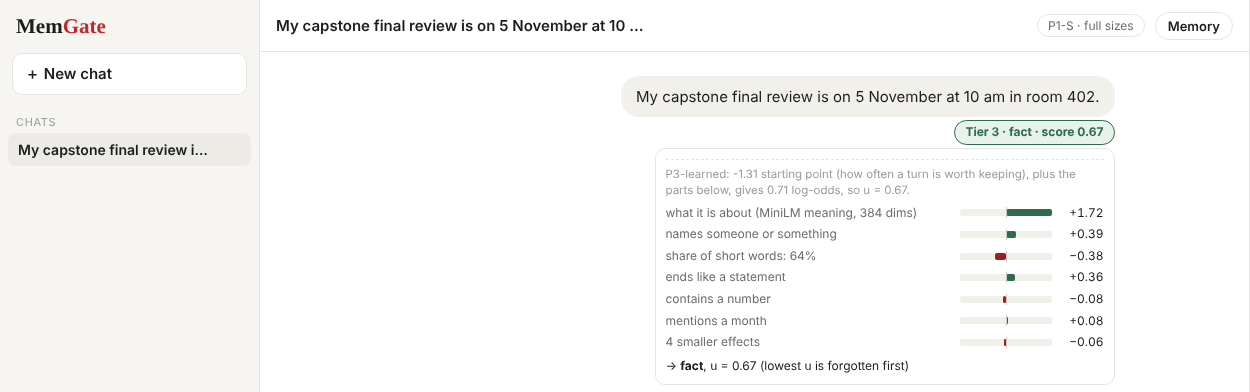
\includegraphics[width=\textwidth]{images/app_tags.png}
\caption{The application tags each message with its tier and score; the
breakdown shows why the learned scorer kept a dated fact.}
\label{fig:apptags}
\end{figure}

\begin{figure}[htbp]
\centering
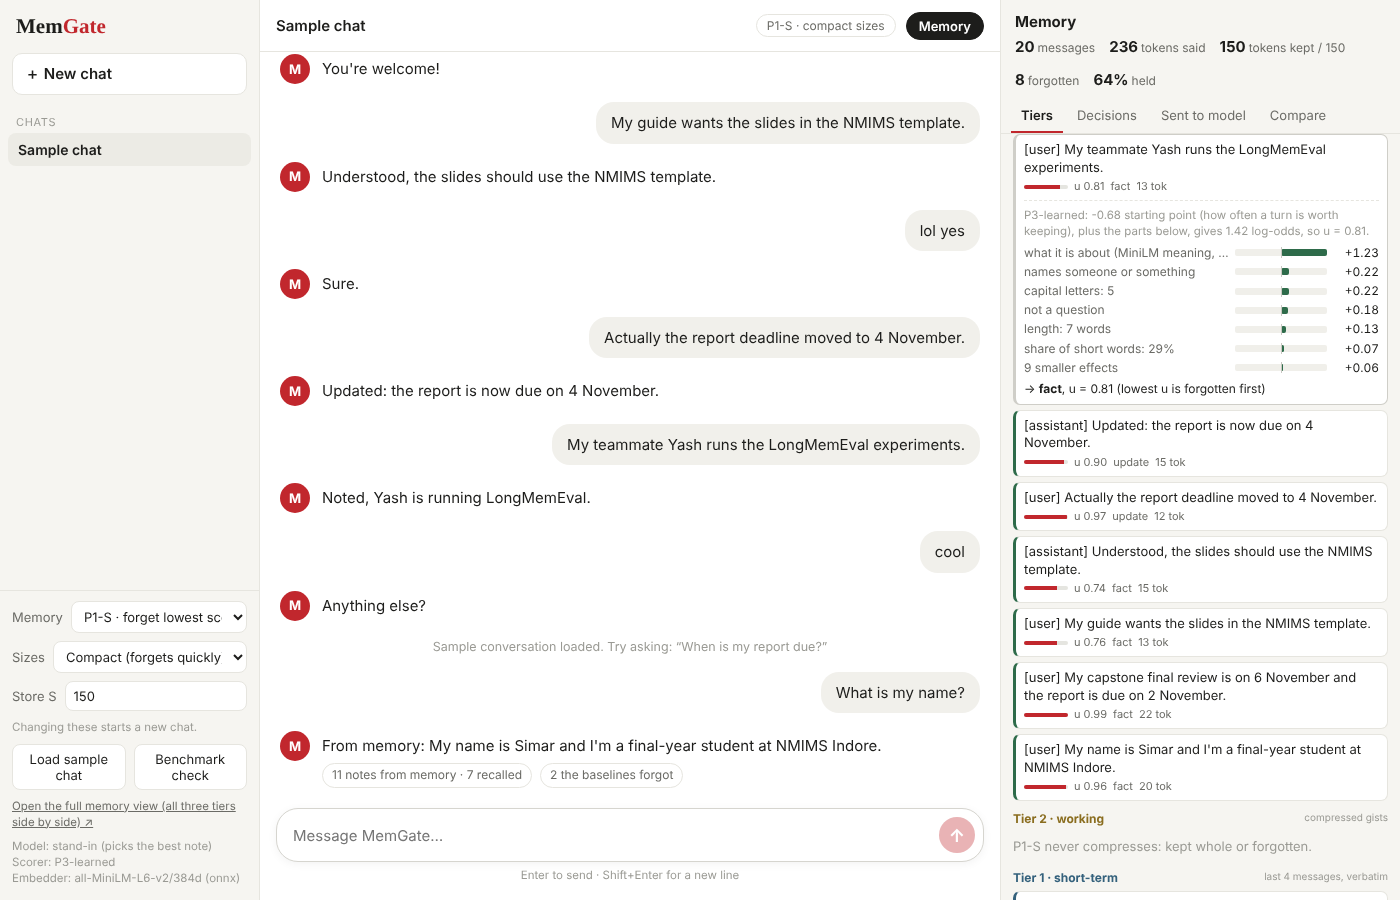
\includegraphics[width=\textwidth]{images/app_memory.png}
\caption{The memory panel: what each tier holds, with the score breakdown of
a stored note.}
\label{fig:appmemory}
\end{figure}

\begin{figure}[htbp]
\centering
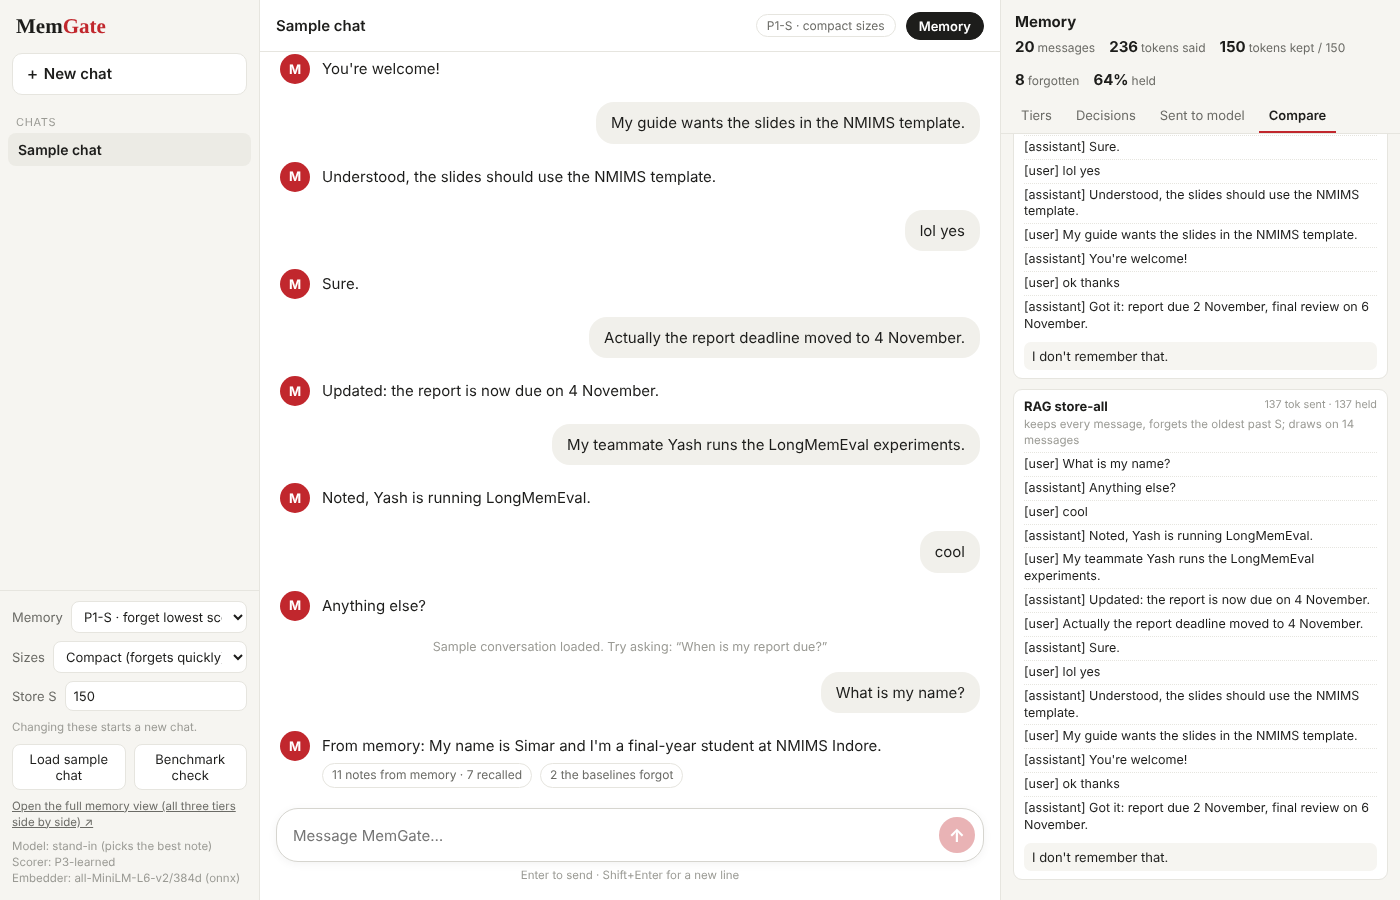
\includegraphics[width=\textwidth]{images/app_compare.png}
\caption{The Compare tab: the same question answered from MemGate, a sliding
window and RAG at the same budgets.}
\label{fig:appcompare}
\end{figure}

\begin{figure}[htbp]
\centering
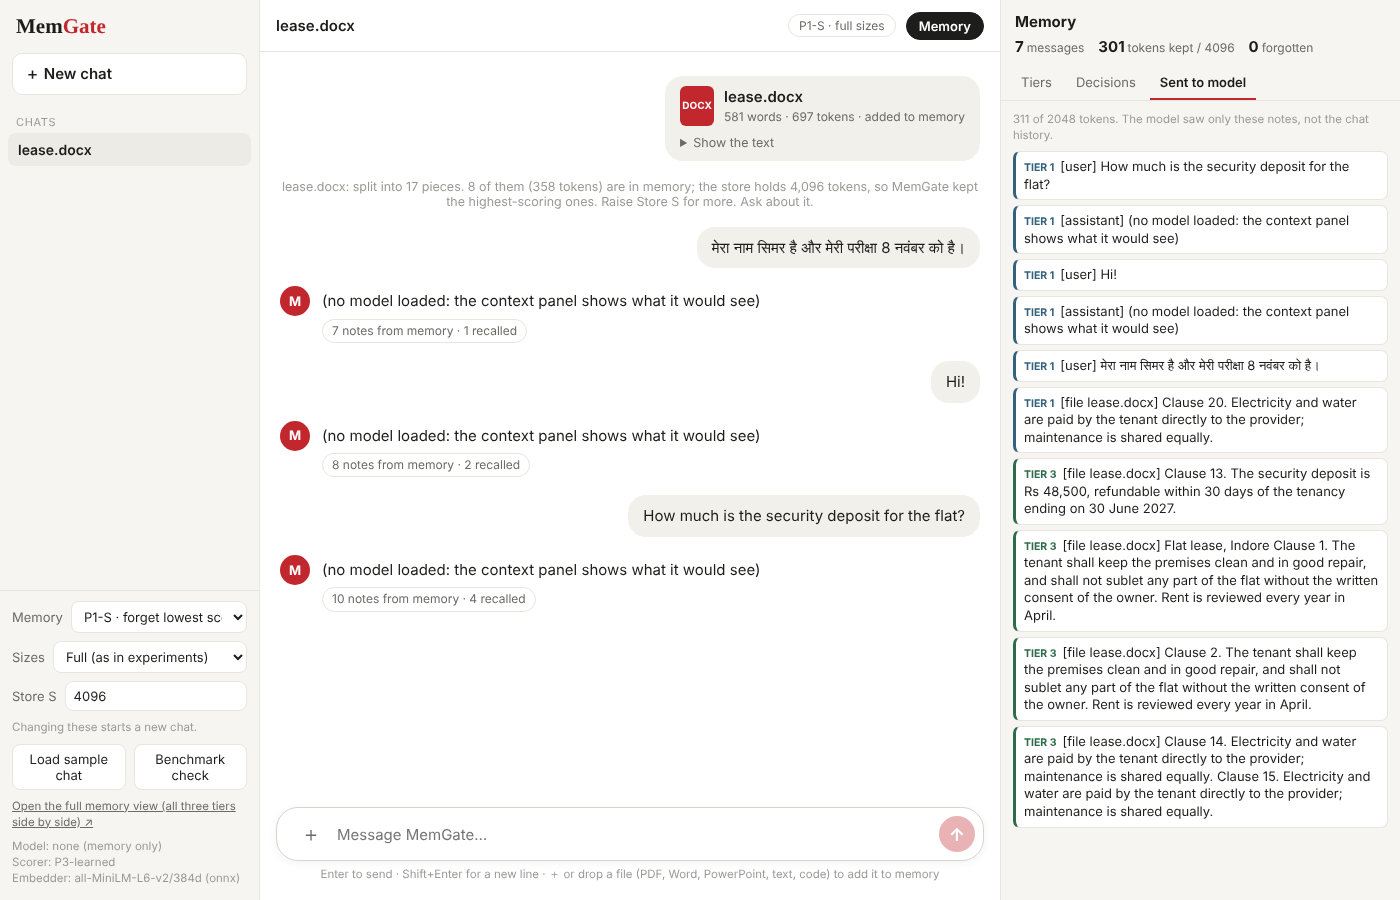
\includegraphics[width=\textwidth]{images/app_upload.png}
\caption[A Word file uploaded into a chat.]{A Word file uploaded into a chat (run without a reply model): the
file is cut into pieces, and the notes sent to the model show the recalled
clauses with their source. A Hindi message is stored the same way.}
\label{fig:appupload}
\end{figure}

\subsection{Server}
The server is a small Python standard-library HTTP server with a JSON API:
\texttt{/api/chat} sends a message, \texttt{/api/upload} adds a file,
\texttt{/api/state} returns the memory panel, \texttt{/api/why} explains a
score, \texttt{/api/rival} runs the comparison, \texttt{/api/bench} the
benchmark check, and \texttt{/api/chats/*} manages saved chats. Request bodies
are size-limited, and the accept queue was raised to 256 after a load test
(Section~\ref{sec:stress}).

\section{Testing and verification}
\label{sec:testing}
Every claim in this report is produced by a script in the repository and is
pinned by a regression test. The test suites cover the library (tiers,
compression, budgets and label-blindness), the scorers, the memory policy, the
reply models, the application endpoints, input handling, the score
explanations and comparison, the rebuilt MemGPT-style and Mem0-style
baselines, and a benchmark check that replays LoCoMo and compares it with the
published numbers. The last full run before this report passed all 453
tests. A GitHub Actions workflow runs every suite, with the real MiniLM
embedder and the LoCoMo data, on each push and pull request.

\section*{Summary}
MemGate is a pure-software memory layer with a three-tier store, a single
scoring site, a hard storage budget and a retrieval-based read path. Its
policies differ in exactly one factor each, so that the experiments isolate
one decision at a time. The learned scorer is a 399-input logistic regression
shipped as plain JSON. The same code runs a chat application that makes every
memory decision visible, and the whole system is held in place by over 450
automated tests.
